\documentclass[11pt]{report}
\usepackage{graphicx}
\usepackage{index}
\usepackage{varioref}
\usepackage{amsmath}
\usepackage{multirow}
\usepackage{theorem} % for examples
\usepackage{alltt}
\usepackage{ulem}
\usepackage{epic,eepic}
\usepackage{boxedminipage}
\usepackage{fancybox}
\usepackage[square]{natbib}
\usepackage{epsfig}
%\usepackage{subfig}
\usepackage{subfigure}
\oddsidemargin 0mm
\evensidemargin 5mm
\topmargin -20mm
\textheight 240mm
\textwidth 160mm



\newcommand{\bold}{\it}
\renewcommand{\emph}{\it}

\makeindex
\theoremstyle{plain}

\newcommand{\nt}[2]{\textrm{#1}_{\framebox[5pt]{\scriptsize #2}}}

\begin{document}
\title{\vspace{-15mm}\LARGE {\bf Final Report}\\[2mm]
of the\\[2mm]
2010 Language Engineering Workshop\\[15mm]
{\huge \bf Models for\\
Synchronous Grammar Induction\\[2mm]
{\tt \Large http://www.clsp.jhu.edu/workshops/ws10/groups/msgismt/}\\[15mm]
Johns Hopkins University\\[2mm]
Center for Speech and Language Processing}}
\author{\large Phil Blunsom,
Chris Callison-Burch,
Trevor Cohn,
Chris Dyer,
Adam Lopez,\\
\large
Jonathan Graehl,
Jonathan Weese,
Jan Botha,
Vladimir Eidelman,
ThuyLinh Nguyen,
Ziyuan Wang, \\
\large Olivia Buzek, Desai Chen}
\normalsize

\maketitle

\section*{Abstract}
The last decade of research in Statistical Machine Translation (SMT) has seen rapid progress. The most successful methods have been based on synchronous context free grammars (SCFGs), which encode translational equivalences and license reordering between tokens in the source and target languages. Yet, while closely related language pairs can be translated with a high degree of precision now, the result for distant pairs is far from acceptable. In theory, however, the ``right'' SCFG is capable of handling most, if not all, structurally divergent language pairs. The 2010 Language Engineering Workshop {\emph Models of Synchronous Grammar Induction for SMT} had the goal to focus on the crucial practical aspects of acquiring such SCFGs from bilingual text. We started with existing algorithms for inducing unlabeled SCFGs (e.g. the popular Hiero model) and then used state-of-the-art unsupervised learning methods to refine the syntactic constituents used in the translation rules of the grammar.

\phantom{.}


\newpage
\section*{Acknowledgments}
The participants at the workshop would like to thank everybody at Johns Hopkins University who made the summer workshop such a memorable --- and in our view very successful --- event. The JHU Summer Workshop is a great venue to bring together researchers from various backgrounds and focus their minds on a problem, leading to intense collaboration that would not have been possible otherwise.

We especially would like to thank Fred Jelinek for heading the Summer School effort and Desir\'ee Cleves for her superhuman ability to keep things running smoothly.

\phantom{.}

\newpage
\section*{Team Members}

\begin{itemize}
\item Phil Blunsom, Team Leader, University of Oxford
\item Chris Callison-Burch, Senior Researcher, Johns Hopkins University
\item Trevor Cohn, Senior Researcher, University of Sheffield
\item Chris Dyer, Senior Researcher, Carnegie Mellon University
\item Adam Lopez, Senior Researcher, University of Edinburgh
\item Jonathan Graehl, Senior Researcher, Information Sciences Institute, USC
\item Jan Botha, Graduate Student, University of Oxford
\item Vladimir Eidelman, Graduate Student, University of Maryland
\item Thuylinh Nguyen, Graduate Student, Carnegie Mellon University
\item Jonathan Weese, Graduate Student, Johns Hopkins University
\item Ziyuan Wang, Graduate Student, Johns Hopkins University
\item Olivia Buzek, Undergraduate Student, University of Maryland
\item Desai Chen, Undergraduate Student, Carnegie Mellon University
\end{itemize}
\tableofcontents


\chapter{Introduction}

Automatically generating high quality translations for foreign texts remains a central challenge for natural language processing research.
Recent advances in statistical machine translation (SMT) has enabled these technologies to move out of research labs an become viable commercial products and useful online tools. \footnote{e.g., translate.google.com, www.systran.co.uk, www.languageweaver.com} 
However these successes have not been uniform; 
current state-of-the-art translation output varies markedly in quality depending on the languages being translated. 
Those language pairs that are closely related language pairs (e.g., English and French) can be translated with high quality, while for distant pairs (e.g., English and Chinese) the result tends to be much lower quality. 
It is tempting to argue that SMT's current limitations can be overcome simply by increasing the amount of data on which the systems are trained. 
However, large scale evaluation campaigns for Chinese~$\rightarrow$~English translation, such as the DARPA GALE program, have not yielded high quality translation despite providing hundreds of millions of words worth of training data. 

\begin{figure}[t]
  \centering 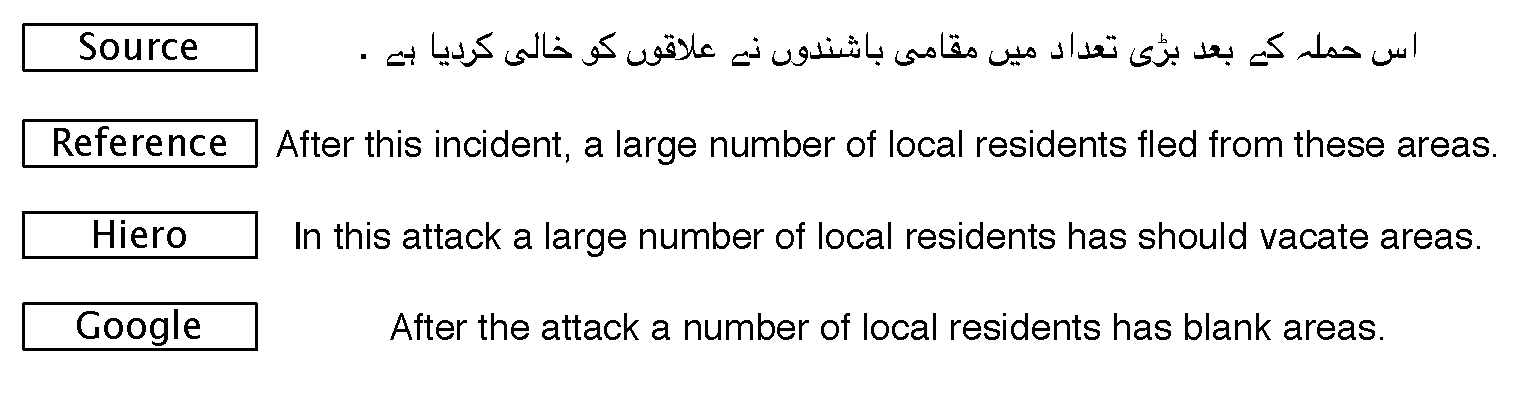
\includegraphics[scale=0.55]{urdu_example_translation.pdf}
\caption{An example Urdu $\rightarrow$ English translation show outputs from both a state-of-the-art Hiero translation model, and Google's translation service.}
\label{fig:intro_urdu_example}
\end{figure}
Figure \ref{fig:intro_urdu_example} shows the current state-of-the-art for translating an Urdu sentence into English.
While a considerable portion of the content of the input Urdu sentence is translated, the end result is still far from being acceptable for an end user. 
%\begin{figure}
%  \centering \includegraphics[scale=1.3]{intro_slides/WhoWroteThisLetter.pdf}
%\caption{The level of structural divergence varies depending on the language pair in question.}
%\label{fig:intro_translation_divergence}
%\end{figure}
Many of the issues faced by SMT systems can be attributed to structural divergence between the languages being translated.
While many researchers are tackling these issues, most proposed solutions are limited by focusing on more expressive models of translation rather than addressing the issue of how, and what, translation units are learnt a priori.


\begin{table}[t]
\centering
  \begin{tabular}{l|rr}
    \hline
    Language & Words &  Domain \\ \hline
    English & 4.5M& Financial news \\
    Chinese & 0.5M & Broadcasting news \\ 
    Arabic &  300K (1M planned)  &  News  \\
    Korean & 54K  & Military \\ \hline
  \end{tabular}
\caption{Major treebanks: data size and domain.}
\label{tab:intro_treebanks}
\end{table}
%\begin{figure}
%  \centering 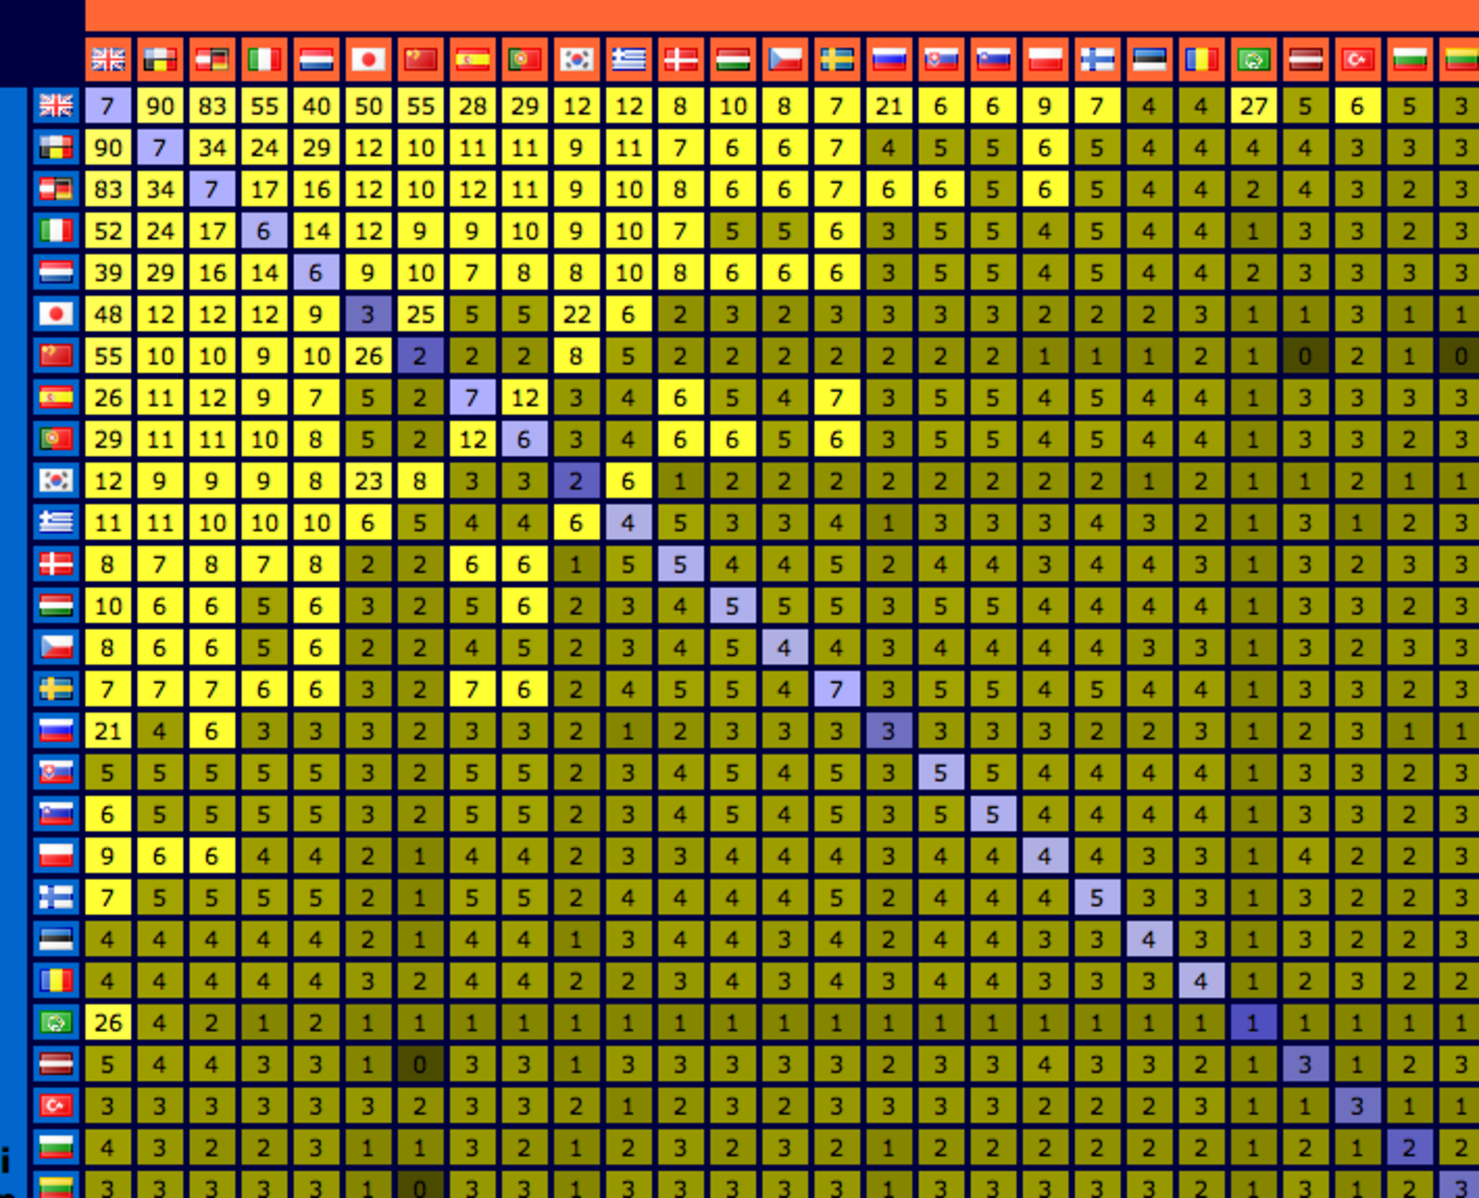
\includegraphics[scale=0.3]{intro_slides/resource_matrix.pdf}
%\caption{A matrix of the number of parrallel words available for various language pairs.}
%\label{fig:intro_parallel_words_matrix}
%\end{figure}

\begin{figure}[t]
  \centering
  \subfigure{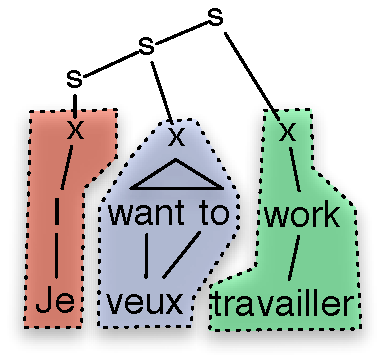
\includegraphics[scale=0.5]{intro_slides/JeVeuxTravailler-Hiero.pdf}}
  \subfigure{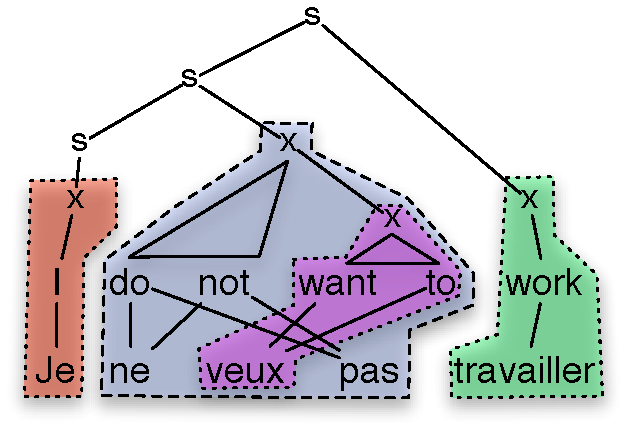
\includegraphics[scale=0.5]{intro_slides/JeNeVeuxPasTravailler-Hiero.pdf}}
\caption{Example derivations using the Hiero grammar extraction heuristics \cite{chiang07hierarchical}.}
\label{fig:intro_hiero}
\end{figure}

\begin{figure}[t]
  \centering
  \subfigure{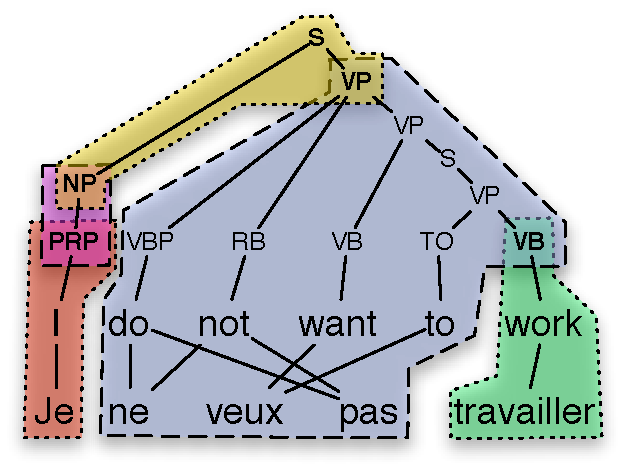
\includegraphics[scale=0.5]{intro_slides/JeNeVeuxPasTravailler-tsg.pdf}}
  \subfigure{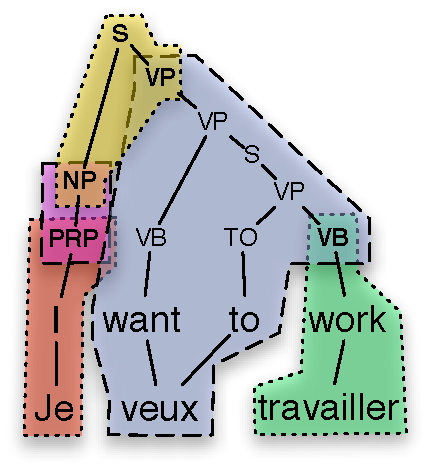
\includegraphics[scale=0.5]{intro_slides/JeVeuxTravailler-tsg.pdf}}
\caption{Example derivations for a Tree Substitution Grammar derived from a parallel corpus parsed with a supervised parser.}
\label{fig:intro_tsg}
\end{figure}

Models which have been most successful for translating between structurally divergent language pairs have been based on synchronous grammars. 
A critical component of these translation models is their {\emph grammar} which encodes translational equivalence and licenses reordering between tokens in the source and target languages. 
There is considerable scope for improving beyond current techniques for automatically acquiring synchronous grammars from bilingual corpora, which seek to find either extremely simple grammars with only one non-terminal or else rely on treebank-trained parsers.
The advantage of using a simple grammar is that no extra annotated linguistic resources are required beyond the parallel corpus.
However these simple grammars are incapable of representing the substitutability of a constituent.
Figure \ref{fig:intro_hiero} displays a synchronous derivation in such a simple grammar.
Richer grammars induced from a parallel corpus annotated with syntax trees overcome the limitations of the simple grammars and provide a far more powerful representation of language structure. 
Figure \ref{fig:intro_tsg} shows a synchronous derivation in for a grammar extracted parallel corpus parsed on the English side.
The limitation of this approach is that the reliance on supervised parses restricts the systems' portability to new target languages (effectively limiting us to translating into/out of English) while enforcing a restrictive notion of linguistic constituency. 
Figure \ref{fig:intro_parallel_words_matrix} shows the number of words in the treebanks available for the most well resourced languages. 
As the performance of supervised parsers is heavily dependent on the amount of training data available, clearly we can expect poorer results when building translation models based upon then for languages other than English.
A further, but more subtle, limitation of these models is the assumption that the particular brand of linguistic structure assigned by a parser (usually a form of phrase structure grammar learnt from the Penn. Treebank) is predominantly isomorphic to that of the input language; an assumption which is rarely true for distantly related language pairs, or even closely related ones.



Clearly there is a need for research into the unsupervised induction of synchronous grammar based translation models.
Previous research has focussed on structured learning approaches requiring costly global inference over translation pair derivations, limiting the ability of these models to be scaled to large datasets \cite{blunsom09bscfg}.
In this workshop we adopted a pragmatic approach of embracing existing algorithms for inducing unlabelled SCFGs (e.g. the popular Hiero model \cite{chiang07hierarchical}), and then used state-of-the-art probabilistic models to independently learn syntactic classes for translation rules in the grammar.
We structured the workshop into three parallel but interdependent streams:

\begin{figure}
  \centering
  \subfigure{\includegraphics[scale=0.5]{intro_slides/JeNeVeuxPasTravailler-hiero-labelled.pdf}}
\caption{Example derivation using the Hiero grammar extraction heuristics where non-terminals have been clustered into unsupervised syntactic categories denoted by $X?$.}
\label{fig:intro_labelled_hiero}
\end{figure}


\paragraph{1) Unsupervised induction of labelled SCFGs}
Inspired by work in monolingual PCFG learning, we have investigated generative models which describe the production of phrase translations in terms of sequences of tokens (or word classes) and their observed contexts.
We simplify the grammar induction problem to first clustering monolingual phrases based upon their distribution over contexts (preceding and following words), and then intersecting these labelled phrases with the Hiero \cite{chiang07hierarchical} SCFG rule extraction heuristics. 
The end result are grammars that produce derivations like that in Figure \ref{fig:intro_labelled_hiero}, where the labels are the unsupervised clusters induced by our context based induction algorithm.

We explored two approaches to the clustering of phrases.
The first was inspired by research in Topic Modelling, in particular Latent Dirichlet Allocation (LDA).
We formulated a model in which each phrase type maintains a distribution over labels, and each context a phrase appears in is generated by first choosing a label, and then generating the context from this labels distribution over contexts.
We extended the basic LDA model to incorporate hierarchical Pitman Yor distributions on the two generating components of the model.
In the second approach we optimised the same model as describe above, but in instead of using non-parametric Bayesian approach to encouraging sparsity in the model, we used the direct Posterior Regularisation technique of \cite{someone}. 

The labelled SCFGs produced by these algorithms generate a subset of the translations licensed by the original Hiero grammars.
While we hope that this restriction guides the model to more acceptable translations, with the inevitable noise present in all automatically induced translation models it is advantageous to allow our models to degrade gracefully to less restrictive grammars.
As such we also explored hierarchical cascades of grammars, each of which was induced with a different number of labels, allowing the translation model to switch between these while incurring a penalty for doing so.

This work on inducing labels for SCFGs formed the core component of the workshop and the base for the following work exploiting these labellings. 
By the conclusion of the workshop we were able to demonstrate that applying these induction techniques leads to improved translations for both Chinese$\rightarrow$English and Urdu$\rightarrow$ translation systems.
Chapter \ref{chap:grammar_induction} describes this work.

\paragraph{2) Decoding with labelled SCFGs}
The second major component of the workshop involved the investigation of improved decoding algorithms for the type of labelled SCFG produced by our induction methods.
Decoding complexity scales quadratically with the number of labels in the grammar.
As such inducing grammars with more than one label significantly increases the time and resources required for decoding.
We explored a number of avenues for reducing this computational burden, including the early pruning items from the search space before language model integration, and coarse-to-fine techniques in which decoding is performed with grammars with progressively more labels and pruning at each step.
We were able to show that each of these techniques could lead to faster decoding without compromising translations performance.
Chapter \ref{chap:decoding} describes this work.

\paragraph{3) Discriminative training labelled SCFG translation models}
The third stream of the workshop focussed on implementing discriminative training algorithms for the labelled SCFG translation models produced by our unsupervised grammar induction algorithms.
Though the existing MERT \cite{och02mert} training algorithm is directly applicable to these grammars, it doesn't allow us to optimise models with large numbers of fine grained features extracted from the labels we've induced.
In order to maximise the benefit from our induced grammars we explored and implemented discriminative training algorithms capable of handling thousands, rather than tens, of features.
The algorithms we explored were Maximum Expected Bleu \cite{smith,li} and MIRA \cite{chiang}.
Chapter \ref{chap:training} describes this work.

The remainder of this introductory chapter provides a formal definition of SCFGs and describes the language pairs that we experimented with.

\section{Synchronous context free grammar} \label{sec:scfg}

A synchronous context free grammar (SCFG, \cite{lewis68scfg}) generalizes context-free grammars to generate strings concurrently in two (or more) languages. A string pair is generated by applying a series of paired rewrite rules of the form, $X \rightarrow \langle \mathbf{e}, \mathbf{f}, \mathbf{a} \rangle$, where $X$ is a non-terminal, $\mathbf{e}$ and $\mathbf{f}$ are strings of terminals and non-terminals and $\mathbf{a}$ specifies a one-to-one alignment between non-terminals in $\mathbf{e}$ and $\mathbf{f}$.
In the context of SMT, by assigning the source and target languages to the respective sides of a probabilistic SCFG it is possible to describe translation as the process of parsing the source sentence, which induces a parallel tree structure and translation in the target language \cite{chiang07hierarchical}.  
Terminal are rewritten as pairs of strings of terminal symbols in the source and target languages.  Additionally, one side of a terminal expansion may be the special symbol $\epsilon$, which indicates a null alignment which permits arbitrary insertions and deletions.
Figure \ref{fig:scfg} shows an example derivation for Japanese to English translation using an SCFG.

\begin{figure}Grammar fragment:
\begin{eqnarray*}
\label{rule:discont}X & \rightarrow & \langle \nt{X}{1}\ \nt{X}{2}\ \nt{X}{3},\ \nt{X}{1}\ \nt{X}{3}\ \nt{X}{2} \rangle  \\
X & \rightarrow & \langle \textrm{\emph{John-ga}},\ \textrm{\emph{John}} \rangle  \\
X & \rightarrow & \langle \textrm{\emph{ringo-o}},\ \textrm{\emph{an apple}} \rangle  \\
X & \rightarrow & \langle \textrm{\emph{tabeta}},\ \textrm{\emph{ate}} \rangle
\end{eqnarray*}
Sample derivation:
\begin{eqnarray*}
\label{derivationt}
& &\langle \nt{S}{1},\nt{S}{1} \rangle \Rightarrow \langle \nt{X}{2},\ \nt{X}{2} \rangle \\
 & \Rightarrow&  \langle \nt{X}{3}\ \nt{X}{4}\ \nt{X}{5},\ \nt{X}{3}\ \nt{X}{5}\ \nt{X}{4} \rangle  \\
 & \Rightarrow &\langle \textrm{\emph{John-ga}}\ \nt{X}{4}\ \nt{X}{5},\ \textrm{\emph{John}}\ \nt{X}{5}\ \nt{X}{4} \rangle \\
 & \Rightarrow &\langle \textrm{\emph{John-ga}}\ \textrm{\emph{ringo-o}}\ \nt{X}{5},\ \textrm{\emph{John}}\ \nt{X}{5}\ \textrm{\emph{an apple}} \rangle \\
 & \Rightarrow &\langle \textrm{\emph{John-ga ringo-o tabeta}},\ \textrm{\emph{John ate an apple}} \rangle
\end{eqnarray*}
\caption{A fragment of an SCFG with a ternary non-terminal expansion and three terminal rules.}
\label{fig:scfg}
\end{figure}

The generative story is as follows. 
In the beginning was the grammar, in which we allow  two types of rules: {\emph non-terminal} and {\emph terminal} expansions. 
The former rewrites a non-terminal symbol as a string of two or three non-terminals along with an alignment $\mathbf{a}$, specifying the corresponding ordering of the child trees in the source and target language. 
Terminal expansion rewrite a non-terminal as a pair of terminal n-grams, where either but not both may be empty. 
Given a grammar, each sentence is generated as follows, starting with the distinguished root non-terminal, $S$. 
Rewrite each frontier non-terminal, $c$, using a rule chosen from our grammar expanding $c$. 
Repeat until there are no remaining frontier non-terminals. 
The sentences in both languages can then be read off the leaves, using the rules' alignments to find the right ordering. 




\newcommand{\p}{\textbf{p}}

\chapter{Nonparametric Models}

In this chapter we describe several closely related Bayesian nonparametric models for inducing categories in a synchronous context-free grammar.  Our nonparametric models are variations on Latent Dirichlet Allocation (LDA) model of \cite{blei:2003}.  Rather than modeling sentences (or sentence pairs), we assume that rule extraction heuristics determine the set of valid constituents and grammar rules, and so our task is only to determine the category labels.  As discussed in the previous chapter, we make the critical assumption that each phrase (or pair), $\p$, can be clustered on the basis of the contexts it occurs in.  We therefore define a generative model of a corpus that consists of collections of contexts (one context collection for each phrase pair type).

\section{Model}

The high-level structure of our model is as follows: each observed phrase (pair), $\p$, consists of a finite mixture of categories, $\theta_{\p}$.  The list of contexts $C_{\p}$ is generated as follows.  A category type $z_i$ is drawn from $\theta_{\p}$, and this generates the observed context, $\textbf{c}_i$, according to a category-specific distribution over contexts types, $\phi_{z_i}$.  Since we do not know the values of $\theta_{\p}$ and $\phi_z$, we place priors on the distributions, to reflect our prior beliefs about the shape these distributions should have and infer their values from the data we can observe.  Specifically, our {\emph a priori} expectation is that both parameters will be relatively peaked, since each phrase, $\p$, should relatively unambiguous belong to particular category, and each category to generate a relatively small number of context strings, $\textbf{c}$.

To encode these prior beliefs, we make use of Pitman-Yor processes \citep{pitman:1997}, which can capture these intuitions and which have already been demonstrated to be particularly effective models for language \citep{teh:2006,goldwater:2006}.

Our models assume a fixed number of categories, $K$. The category type, $z \in \{ 1 , 2 , \ldots , K \}$, is generated from a PYP with a uniform base distribution:
\begin{align*}
z &| \p & \sim \theta_{\p} \\
\theta_p &| a_{\p},b_{\p},K & \sim \textrm{PYP}(a_{\p},b_{\p},\textrm{Uniform}(K))
\end{align*}
\noindent Alternatively, we used hierarchical PYP process which shares statistics about the use of categories across phrases:
\begin{align*}
z &| \p & \sim \theta_{\p} \\
\theta_{\p} &| a_{\p},b_{\p} & \sim \textrm{PYP}(a_{\p},b_{\p},\theta_0) \\
\theta_0 &| a_0,b_0,K & \sim \textrm{PYP}(a_0,b_0,\textrm{Uniform}(K))
\end{align*}

\noindent Each category $z$ token then generates the context $\textbf{c}_i$. We again model this using a PYP, which will tend to cluster commonly used contexts across phrases into a single category. Additionally, by using hierarchical PYPs, we can smooth highly specific contexts by backing off to less specific contexts (e.g., composed of fewer words or word classes).

The most basic version of our model uses a uniform prior base distribution over contexts:

\begin{align*}
\textbf{c} |& z & \sim \phi_z \\
\phi_z |& a_z,b_z & \sim \textrm{PYP}(a_z,b_z,\textrm{Uniform}(|V|^2))
\end{align*}

\noindent TODO. For contexts with more than a single word on either side, we typically backed off from a 

\begin{align*}
\textbf{c} |& z & \sim \phi_z \\
\phi_z |& a_z,b_z, \phi_0 & \sim \textrm{PYP}(a_z,b_z,\phi_0(\cdot|z) \times \textrm{Uniform}(|V|^2)) \\
\phi_0 |& a_0,b_0 & \sim \textrm{PYP}(a_z,b_z,\phi_0(\cdot|z))
\end{align*}

\noindent Figure~\ref{fig:np_plate} shows a plate diagram for the model.

\begin{figure}
\begin{center}
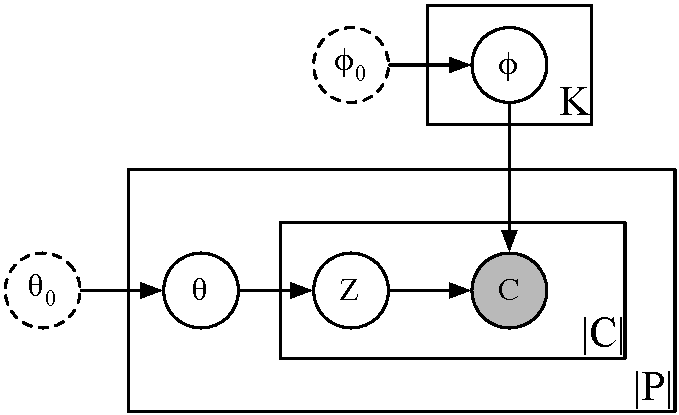
\includegraphics[scale=0.75]{pyp_clustering/np_plate.pdf}
\vspace{-0.3cm}
\end{center}
\caption{Plate diagram for the nonparametric clustering model (hyperparameters omitted).  Dashed circles indicate variables that may not be present in every model.}
\label{fig:np_plate}
\end{figure}

\subsection{Inference}

Inference in this model was performed using Gibbs sampling \citep{geman:1984}, with the continuous parameters ($\theta_{\p}$, $\phi_z$, etc.) integrated out.  For the experiments reported below, we sampled for 1000 iterations, initializing by assigning every context in a phrase entirely to a random category.  New values for the PYP hyperparameters were resampled using slice sampling every 10 samples \citep{neal:2000,johnson:2009}. The final sample was used to estimate $p(z|\textbf{c},\p)$, and each phrase occurrence was labelled with the $z$ that maximized this probability (TODO check this).

\section{Experiments}

\subsection{Number of categories}

\subsection{Context types}



\chapter{Training}

An integral part of constructing a state-of-the-art machine translation system is the training procedure. The goal of training is to optimize the model parameters to maximize translation quality on some metric, where the parameters are the weights associated with the features we use in our model, and the metric is BLEU. 

The most common approach to training is Minimum Error Rate Training (MERT), which tunes the parameters to minimize error according to an arbitrary error function. Thus, in our case this is equivalent to saying that it maximizes the 1-best translation under the BLEU metric. MERT is a log-linear model which allows us to combine different features in order to find the best target translation $e*$ for a input source $f$:
$$e* = \arg\max e p(e|f) = argmax_e \sum_{k=1}^K w_kh_k(e,f)$$

where $h_k(e,f)$ is a feature associated with the translation of $f$ to $e$, and $w$ is the weight associated with that feature. Unfortunately, MERT has been empirically unable to extend beyond optimization of a handful of features, thus necessecitating dense features. Theses features typically include:

\begin{itemize}
\item rule relative frequency $P(e|f)$
\item target $n$-gram language model $P(e)$
\item `pass-through' penalty when passing a source word to the target side untranslated
\item lexical translation probabilities $P_{lex}(\overline{e}|\overline{f})$ and $P_{lex}(\overline{f}|\overline{e})$
\item count of the number of times that arity-0,1, or 2 SCFG rules were used 
\item count of the total number of rules used
\item source word penalty
\item target word penalty
\item count of the number of times the glue rule is used 
\end{itemize} 

However, after the creation of the refined grammars which have been described in the previous sections, we have additional information available to us which we would like to leverage in order to improve translational performance. The way in which we would like to utilize this informaiton is by extracting it as features for our model. For instance, some features of particular instance may be:

\section{Feature Extraction}
There are a number potentially useful features we could extract from the refined grammars, such as:
\begin{itemize}
\item Source Syntactic Features
\item Target Syntactic Features
\item Source Context Features
\item OOV
\item Glue Rule
\item Morphology
\end{itemize}


\subsection{Source Syntactic Features}

Recent work with syntax-based systems which parse the source side with a previously trained supervised parser has shown that utilizing syntactic patterns can lead to substantial improvements. Such patterns can be especially useful in capturing long-range reordering patterns, and other high-level phenomena that we are otherwise unable to leverage. Figure~\ref{fig:synt_feat1} shows an example syntactic pattern, which captures the application of rule $X_{12}$ expanding to $X_{17}X_{25}$. Although this rule may not be particularly interesting, as the translation stays monotonic. 

\begin{figure}[h]
	\centering
		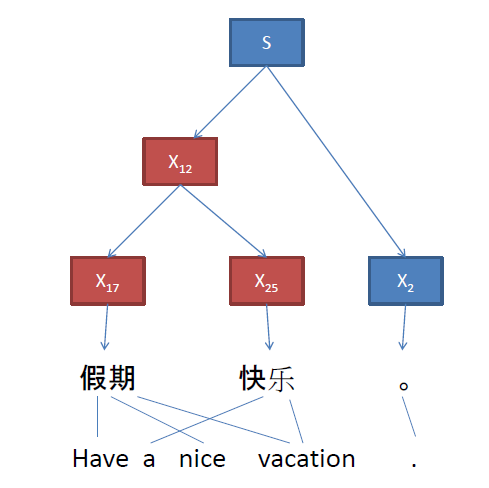
\includegraphics[scale=0.5]{training_img_files/synt_feat1.PNG}
	\caption{Syntactic Feature}
	\label{fig:synt_feat1}
\end{figure}

A more interesting example is presented in Figure~\ref{fig:synt_feat2}, where we can observe a large reodering taking place as $X_1$ expands to $X_6X_19$ and the latter moves to the left of the former.

\begin{figure}[h]
	\centering
		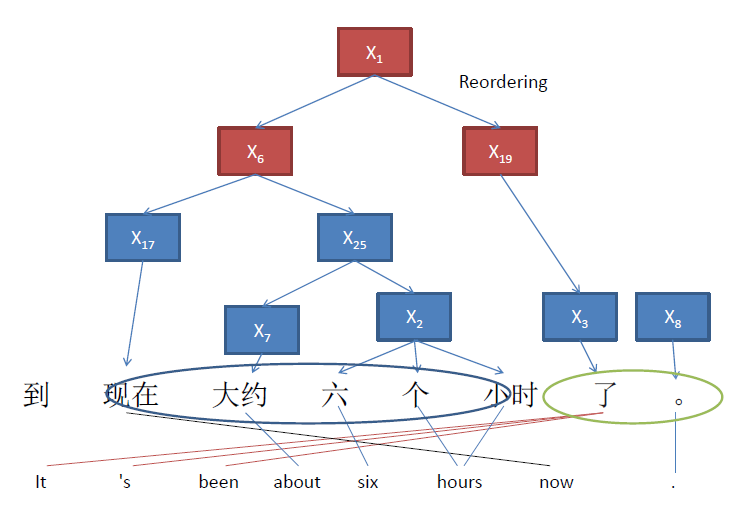
\includegraphics[scale=0.5]{training_img_files/synt_feat2.PNG}
	\caption{Syntactic Reordering Feature}
	\label{fig:synt_feat2}
\end{figure}


\subsection{OOV}
Although we will always encounter Out-of-Vocabulary terms, we may be able to utilize the finer-grained categories to capture syntactic distribution patterns associated with each category to learn how to process the OOV terms. This may be particularly useful for numbers, nouns such as Proper names, or certain adjectives, which tend to cluster togther, as shown in Figure~\ref{fig:oov_feat}.

\begin{figure}[h]
	\centering
		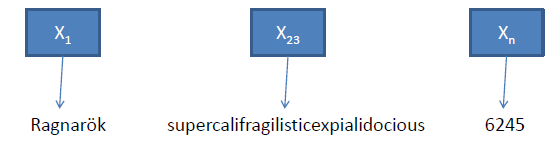
\includegraphics[scale=0.5]{training_img_files/oov_feat.PNG}
	\caption{OOV Feature}
	\label{fig:oov_feat}
\end{figure}

\subsection{Glue Rule}
In our current system, we have one dense feature for all Glue rule applications, however, there are in fact two seperate applications which we would like to distinguish. The first occurs when a top-level $S$ node expands to one of the $X_n$ categories in the grammar, as shown in Figure~\ref{fig:glu_feat}. The second occurs when an $S$ expands to another $S$ and one of the $X_n$ categories, as in Figure~\ref{glu_feat2}. Both of these features attempt to capture the high-level derivation structure of a sentence. 

\begin{figure}[h]
	\centering
		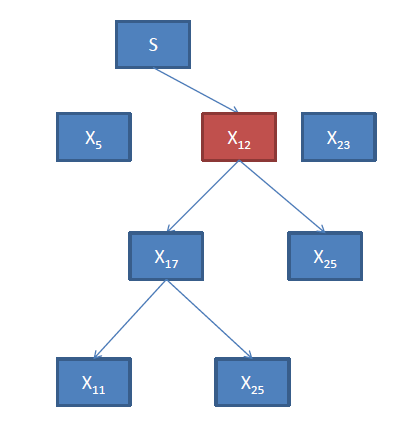
\includegraphics[scale=0.5]{training_img_files/glu_feat.PNG}
	\caption{Glue Rule Expansion Feature}
	\label{fig:glu_feat}
\end{figure}


\begin{figure}[h]
	\centering
		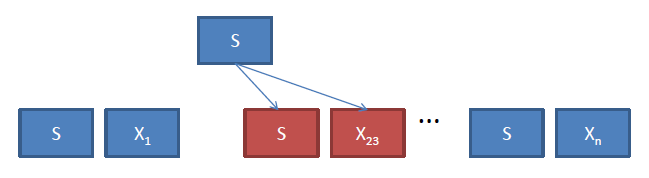
\includegraphics[scale=0.5]{training_img_files/glu_feat2.PNG}
	\caption{Glue Rule Combination Feature}
	\label{fig:glu_feat2}
\end{figure}

\subsection{Backoff}
Given that we have achieved significant gains from incorporating the hierarchical-bacoff feature as a dense feature, it may also be useful to add a sparser version in additional to or in place of the feature we currently use, of the form shown in Figure~\ref{fig:back_feat}.


\begin{figure}[h]
	\centering
		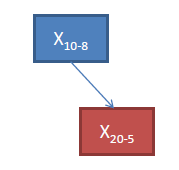
\includegraphics[scale=0.5]{training_img_files/back_feat.PNG}
	\caption{Backoff Feature}
	\label{fig:back_feat}
\end{figure}

\section{Training Algorithms}

As we are interested in incorporating numerous features into our model to directly help translation, we want to perform discriminative training. Given the fact that MERT is unable to optimize the sparse features we are interested in, in this workshop we investigated two alternative methods which allow us to train a model with a high dimensional feature space. The two approaches were the Margin Infused Relaxed Algorithm (MIRA) and Expected BLEU. All three optimization algorithms perform inference over the hypergraph, but as Table~\ref{tab:comp} shows, they are performing in quite different ways. MERT aims to optimize parameters to maximize the 1-best BLEU, or alternatively to minimize the error, by constructing a piece-wise linear error surface from the entire tuning set and performing a line search in order to find the appropriate weights. The primary limitation of this, which is responsible for its inability to scale, is the unknown diretion of the line search. When done in a handful of dimensions, random directions work relatively well, however, as we increase the feature space this becaomes a severe problem. 

Expected BLEU training, explained in detail in Section~\ref{sec:exp_bleu} is a probabilistic method which can be seen as an attempt to address some of these shortcomings. If instead of maximizing the 1-best hypothesis, as we do with MERT, we try to maximize the expected BLEU over all the hypotheses, we create a continuous, and therefore differentiable function for optimization which allows us to use gradient-based methods, such as L-BFGS. 

MIRA training, on the other hand, is a large-margin based training method, which attempts to miminimze the loss augmented score of hypotheses against some reference translation in an online fashion. In order to do so, we need to solve a Quadratic optimization problem with linear constraints, which can be handled by a technique such as Sequential Minimal Optimization (SMO). The foremost downside of this approach is the approximation of the reference that needs to take place for the training to proceed. Since the MT grammar may not contain the necessary rules to produce the correct reference translation, therefore making the translation unreachable, we need to rely on an approximation of the reference. Previous work has explred various approaches for this, such as updating toward the model 1-best, or oracle 1-best. Another possibility is that there may be multiple derivations which lead to the same translation, therefore creating ambiguity regarding which rules, and features should be updated towards. We will expand on this in Section~\ref{sec:mira}.

\begin{table*}[htb]
	\centering
		\begin{tabular}{|c|c|c|c|} 
			& MERT & MIRA & Expected BLEU \\ \hline
			Type & 1-best & Margin-based & Probabilistic \\ \hline
			Objective & Minimize error & Minimize loss augmented score & Minimize expected error \\ \hline
			Optimization & Line search & QP & Gradient Based \\ \hline
			Limitations & Direction of search unknown & Approximation of reference & Approximate expectation \\ \hline
		\end{tabular}
	\caption{Training Comparison}
	\label{tab:TrainingComparison}
\end{table*}

\section{Margin Infused Relaxed Algorithm}
\label{sec:mira}

MIRA was first introduced in 2003 by Crammer and Singer for the multi-class classification problem as a perceptron like algorithm, with the additional of a classifcation margin to reduce generalization error. This was later expanded by Taskar to structured value prediction problems, such as dependency parsing. It was notably applied to machine translation by Watanabe, and then Chiang, on whose work we build here.

\subsection{Learning Algorithm}
The basic online learning algorithm proceeds as in Algorithm X. We go through the data for $n$ iterations, and during each iteration we go through all our data points and update the weight vector after each example. We then use the new weight vector to process the next example, and so on, until we reach some convergence criteria. After convergence, we average over the weight vectors to produce a final weight vector which we can use to process new examples. The averaging of the weight vector is done to reduce overfitting, and has proved effective in previous applications. 

When performing inference over the hypergraph, each edge in the hypergraph corresponds to a partial translation and has associated with it a decomposable score $s$:
$$s(edge_i) = w*f(edge_i)$$
which is comprised of the features on that edge and the current weight vector. These can then be added together to produce the score associated with a specific hypothesis translation:
$$\sum_{edge \in derivation} s(edge)= S(e) $$

We also compute a decomposable loss at each edge,which is the approximate BLEU score of the partial hypothesis on the edge. 
What we want is to learn $w$ such that the correct output translation is given a higher score than the incorrect ones. The MIRA update does this optimization by keeping the norm of the change of the weights as small as possible
$$ min ||w_{i+1} - w_i||$$
subject to the margin constraints, which take the following form:
$$ s(x,y) - s(x,z) \geq Loss(y,z), \forall{z} \in label(x)$$

Essentially, these margin constraints force us to create a margin between the correct instance y, and the incorrect instance z which is at least as large as the Loss of z.




\subsection{Oracle Extraction}
In multi-class classification, we can form the constraint set by looking at all the possible labels of x, however, in structured prediction, this becomes infeasible. Thus, in practice previous work has resorted to approximating the constraint set by performing k-best extraction over the trees in dependency parsing, or translations in MT, using only these top $k$ labels as constraints in training. This leads to the modified training algorithm of k-best MIRA, described in Algorithm Y. 

For MT, recent work has shown significant improvements from obtaining three different sets of k-best lists. The first is the model k-best
$$w*f(e) $$
 the second is the model+BLEU, also referred to as the oracle or hope hypothesis The first translation in this k-best set is the oracle translation toward which we update:
 $$w*f(e) + BLEU $$
 and the third is model-BLEU, or the feat hypothesis:
 $$w*f(e) - BLEU $$
 

The impetus behind updating toward towards a combination of the model and BLEU as the oracle translation is that some translations may have an excellent BLEU score, but a distant model score from the area in which most good translation reside, and parroting Voltaire, we do not want to the perfect to be the enemy of the good. 
 
The reasoning behind the third set of k-best lists is that the constraints we care most about for learning are the ones where our system believes the hypothesis is a good one, and thus assigns it a high score, while the BLEU score is poor, thus proving in fact to be a poor translation. 

\subsection{Online Updating}
In order to efficiently train an online learning, significant modifications were necessary to our existing parallelization framework. As updating the weight vector after each example may be inadvisable since the weights could suffer significant jumping around, we could perform mini-batch updating, where weights are only updated after a certain amount of examples have been processed. An alternative which is similar in spirit is to run several learners in parallel, and have them share their k-best hypotheses sets between themselves, in order for each learner to incorporate more information at each update. Figure ~\ref{fig:update1} presents three learners receiving a sentence in parallel. Each learner has its own MIRA trainer and decoder, with its own feature weight vector. In Figure ~\ref{fig:update2} we see Learner 1 completing its decoding of the sentence with its current weight vector, and generating the three k-best lists as described above. It then uses these to update its weights for decoding the next sentence. In Figure ~\ref{fig:update3} we see that both Learner 1 and 2 have completed decoding and generate their respective k-best lists, and these are passed to Learner 3 in order for it to incorporate them, as well as it's own set of k-best lists, when it updates its weight vector.

\begin{figure}[h]
	\centering
		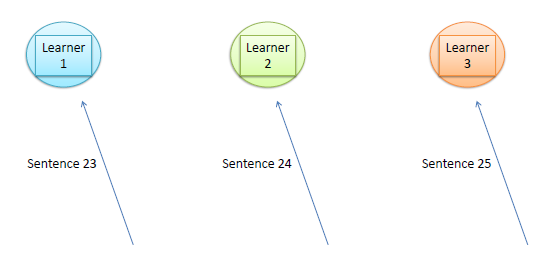
\includegraphics[scale=0.5]{training_img_files/update1.PNG}
	\caption{Online Udpating 1)}
	\label{fig:update1}
\end{figure}


\begin{figure}[h]
	\centering
		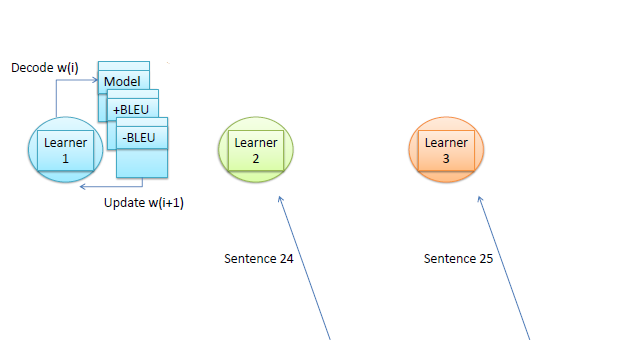
\includegraphics[scale=0.5]{training_img_files/update2.PNG}
	\caption{Online Udpating 2)}
	\label{fig:update2}
\end{figure}


\begin{figure}[h]
	\centering
		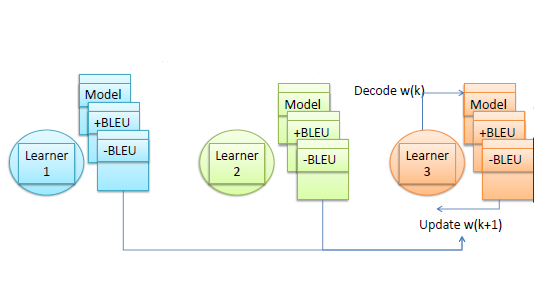
\includegraphics[scale=0.5]{training_img_files/update3.PNG}
	\caption{Online Udpating 3)}
	\label{fig:update3}
\end{figure}

\section{Expected BLEU}
\label{sec:exp_bleu
}
\section{Accomplishments}
During the workshop, we succeeded in completely implementing MIRA and Expected BLEU training in Joshua and cdec, two state-of-the-art open source decoders. This includes the ability to extract oracles from the lattices, as well as the online updating parallelization architecture. Due to a lack of time and resources, we were unfortunatley unable to run the full suite of experiments which we had hoped for, but we leave these as immediate future work.

\section{Future Work}
The first set of experiments concerns a standardized comparison of MIRA and Expected BLEU training, using as-close-as-possible simliar grammas, features, and data sets. To the best of our knowledge, a systematic comparison of these two popular training algorihtms has not been performed, and would be of benefit to the community. 

Second, we are interested in the language invariability of the parameters, number of iterations, and so forth for these algorthims. 




\bibliographystyle{apalike}
\bibliography{biblio}

\printindex

\end{document}
